\documentclass[aspectratio=169]{beamer}
\usepackage{tikz}
% numbering=none,counter,fraction - frame number at bottom right
\usetheme[block=fill,numbering=none,progressbar=foot]{metropolis}           % Use metropolis theme

\definecolor{RoyalBlue}{cmyk}{1, 0.50, 0, 0}
\definecolor{BgBlue}{cmyk}{1, 0.5, 0,0.8}

\setbeamercolor{progress bar}{fg=RoyalBlue!100, bg=RoyalBlue!30}
\setbeamercolor{frametitle}{bg=BgBlue!100}
\title{AIOLI - AI Open Lab Initiative}
\date{\today}
%\author{Tobias Weis - weis@ccc.cs.uni-frankfurt.de}
\author{\texorpdfstring{\url{[mundt,weis]@ccc.cs.uni-frankfurt.de}}{Tobias Weis}}
\institute{Systems Engineering for Computer Vision}

%%%%%%%%%%%%%%%%%%% TITLE RIGHT
\makeatletter
\setbeamertemplate{title page}{

  \begin{minipage}[b][\paperheight]{\textwidth}

    %\centering
    \raggedleft
    \ifx\inserttitlegraphic\@empty\else\usebeamertemplate*{title graphic}\fi
    \vfill%
    \ifx\inserttitle\@empty\else\usebeamertemplate*{title}\fi
    \ifx\insertsubtitle\@empty\else\usebeamertemplate*{subtitle}\fi
    %\usebeamertemplate*{title separator}
    \ifx\beamer@shortauthor\@empty\else\usebeamertemplate*{author}\fi
    \ifx\insertdate\@empty\else\usebeamertemplate*{date}\fi
    \ifx\insertinstitute\@empty\else\usebeamertemplate*{institute}\fi
    \vfill
    \vspace*{1mm}
  \end{minipage}
}

\setbeamertemplate{title}{
  \raggedleft%
  \linespread{1.0}%
  \inserttitle%
  \par%
  \vspace*{0.5em}
}
\setbeamertemplate{subtitle}{
  \raggedleft%
  \insertsubtitle%
  \par%
  \vspace*{0.5em}
}
\makeatother

%%%%%%%%%%%%%%%%%%%%%%%

\begin{document}


{\usebackgroundtemplate{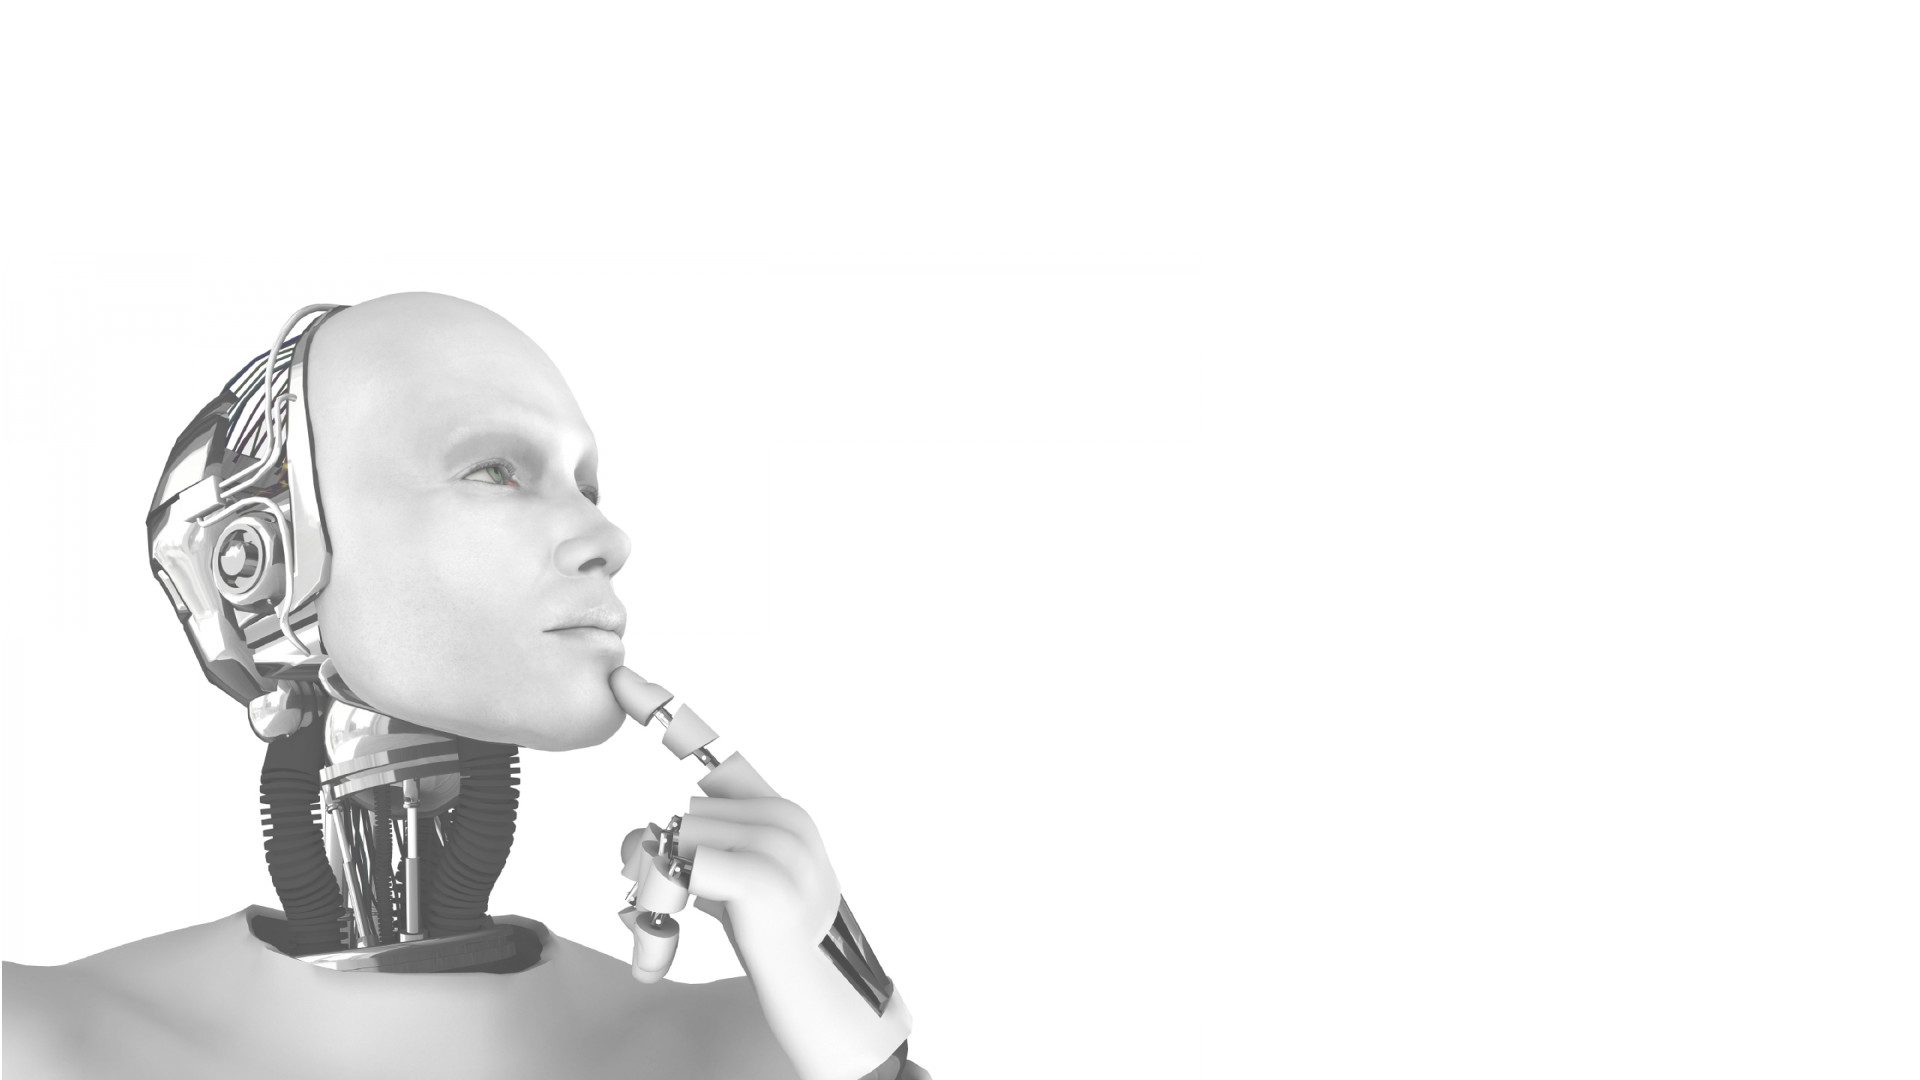
\includegraphics[width=\paperwidth]{images/ai_bg.jpg}}
\maketitle}

%\usebackgroundtemplate{
%}

%%%%%%%%%%%%%%%%%%%%%%%%%%%%%%%%%%%%%%%%%%%%%%%%%%%%%%%%%%%%%%%%%%%%%%%%%%%%%%%%
%                       DEFINITIONS
%%%%%%%%%%%%%%%%%%%%%%%%%%%%%%%%%%%%%%%%%%%%%%%%%%%%%%%%%%%%%%%%%%%%%%%%%%%%%%%%
\section{Before we start}
	\begin{frame}{Before we start}
		To participate in the hands-on coding session afterwards, please:
		\begin{itemize}
			\item Make sure you've got Python 2.7 installed
			\item Download the dataset: \href{http://bit.ly/2i0LkQs}{ \texttt{bit.ly/2i0LkQs}}
			\item Download the example code: \href{https://github.com/aioli-ffm/music-projects}{\texttt{github.com/aioli-ffm/music-projects}}
			\item Follow the instructions in: \texttt{simple\_music\_classifier/README.md}
		\end{itemize}
	\end{frame}

\section{Agenda}
	\begin{frame}{Agenda}
		\tableofcontents
	\end{frame}

\section{Task and Data}
	\begin{frame}{Our task}
		Our Task: Teaching a computer program to distinguish musical genres
		\vfill
		\texttt{Audience participation: Can you guess the genre?}
		\vfill
	\end{frame}

	\begin{frame}{Our data}
		\begin{block}{What data will we feed into our program?}
			From what we've discovered so far: 2s of audio are sufficient to distinguish musical genres.
			We will be using 2s long slices of audio.
		\end{block}

		\bigskip

		\begin{block}{What data do we expect the program to produce?}
			A probability for each genre the program knows; How likely the program thinks it is a given input matches
			a certain musical genre.
		\end{block}

	\end{frame}

	\begin{frame}{Input representation}
		\begin{columns}[T]
		    \begin{column}{.5\textwidth}
		    	\begin{block}{Sampling of continous audio}
					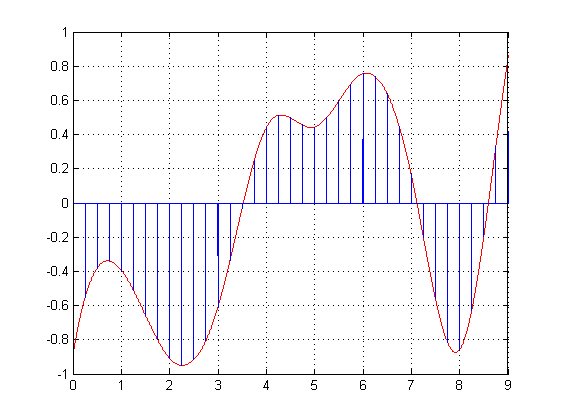
\includegraphics[width=\textwidth]{images/signal_sampling.png}
		   		\end{block}
		    \end{column}
		    \begin{column}{.5\textwidth}
		    	\begin{block}{Audio file in time domain}
		    		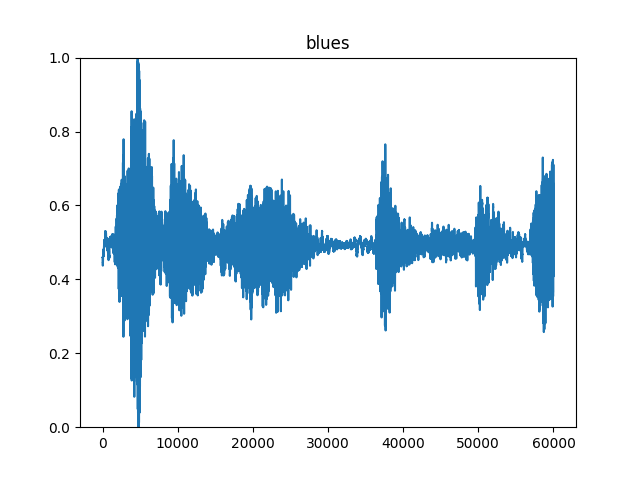
\includegraphics[width=\textwidth]{images/cat_blues.png}
		    	\end{block}
		    \end{column}
		  \end{columns}
	\end{frame}

	\begin{frame}[fragile]
		\frametitle{Input representation}
		\begin{columns}[T]
		    \begin{column}{.5\textwidth}
		    	\begin{block}{Sampling of continous audio}
					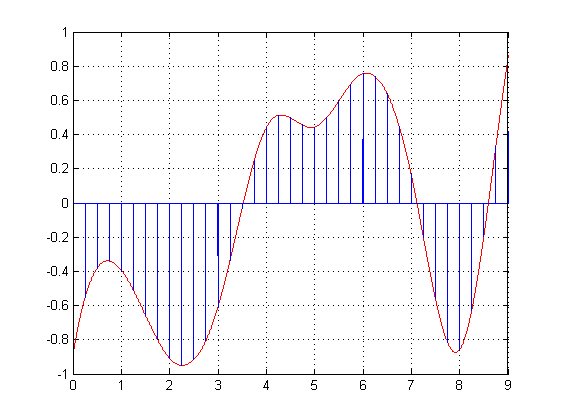
\includegraphics[width=\textwidth]{images/signal_sampling.png}
		   		\end{block}
		    \end{column}
		    \begin{column}{.5\textwidth}
		    	\begin{block}{Representation as list of samples}
		    		\begin{verbatim}
		    			[ -18176, -50090, 61573,
		    			  -27710, -55937, 57950,
		    			  -16483, -32160, 49011,
		    			  ...
		    			  -12336, 13795, -59832 ]
		    		\end{verbatim}
		    	\end{block}
		    \end{column}
		  \end{columns}
	\end{frame}

	\begin{frame}{GTZAN dataset}
		We will be using the GTZAN dataset:
		\vfill
		\begin{itemize}
			\item 10 musical genres
			\item 100 audio files
			\item 30s per audio file
		\end{itemize}
		\vfill
		$\rightarrow$ 30000s of labeled audio
	\end{frame}

\section{Basics of neural networks}
	\begin{frame}{What is a neural network?}
		\begin{columns}[T]
		    \begin{column}{.5\textwidth}
		    	\begin{block}{A real neuron}
					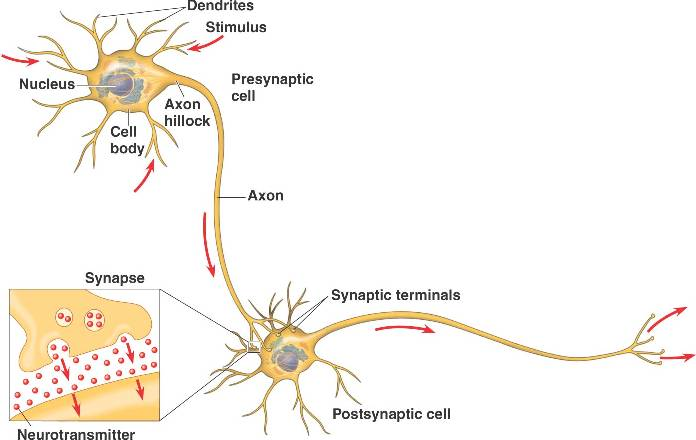
\includegraphics[width=0.95\textwidth]{images/neuron.jpg}
		   		\end{block}
		    \end{column}
		    \begin{column}{.5\textwidth}
		    	\begin{block}{An artificial neural network}
		    		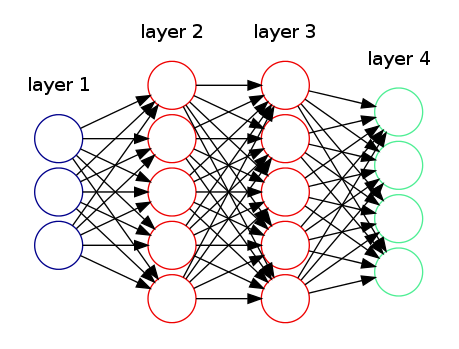
\includegraphics[width=0.95\textwidth]{images/nn.png}
		    	\end{block}
		    \end{column}
		  \end{columns}
	\end{frame}

	\begin{frame}{Neurons and activation}
		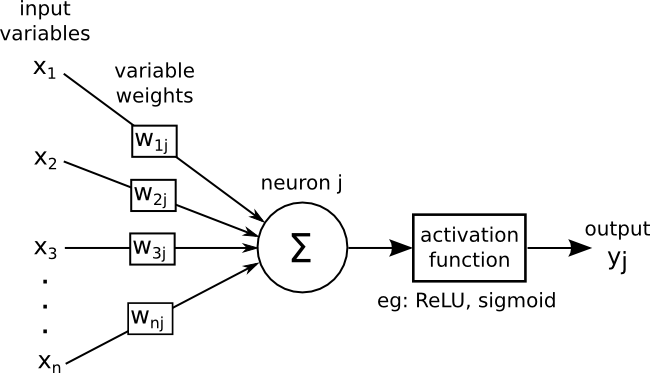
\includegraphics[width=0.8\textwidth]{images/activation.png}
	\end{frame}

	\begin{frame}{Training an NN}
		An output neuron's activation is influenced by:
		\begin{itemize}
			\item The activations of neurons that feed into it
			\item The weights of incoming connections
			\item The bias
			\item The activation function
		\end{itemize}
		Given an activation function, how should we change the weights and biases to improve the output activation? \\
		What does it mean to improve?
	\end{frame}

	\begin{frame}{Backpropagation and Optimization}
		\begin{columns}[T]
			\begin{column}{.5\textwidth}
		    	\begin{block}{Optimization and Loss}
		    		We...
		    		\begin{itemize}
		    			\item will put training data through the neural network
		    			\item need to know how bad our output is, therefore:
		    			\item define a loss function which judges the output
		    			\item will try to minimize this loss function
		    		\end{itemize}
		    	\end{block}
		    \end{column}
		    \begin{column}{.5\textwidth}
		    	\begin{block}{Backpropagation}
					\begin{itemize}
						\item Steps backwards through the network
						\item If we change a weight or bias by a tiny amount, how will the loss function change?
						\item Computes in which direction the weights and biases should change to minimize loss
					\end{itemize}
		   		\end{block}
		    \end{column}
		  \end{columns}
	\end{frame}

	\begin{frame}{Why we need frameworks}
		Frameworks are handy for:
		\begin{itemize}
			\item Abstracting away backpropagation and optimization
			\item Doing computionally intensive work efficiently
			\item Parallelization using GPUs
			\item Minimizing potential error sources
		\end{itemize}
	\end{frame}

	\begin{frame}{GPU vs CPU for NNs}
		\begin{columns}[T]
		    \begin{column}{.5\textwidth}
		    	\begin{block}{Speedup through parallelization}
		    		\begin{itemize}
		    			\item Training NNs can be massively parallelized
		    			\item Modern GPUs are basically parallel processing units
		    			\item We can achieve huge speedups by using GPUs
		    		\end{itemize}
		   		\end{block}
		    \end{column}
		    \begin{column}{.5\textwidth}
		    	\begin{block}{Nvidia GPU vs CPU performance}
		    		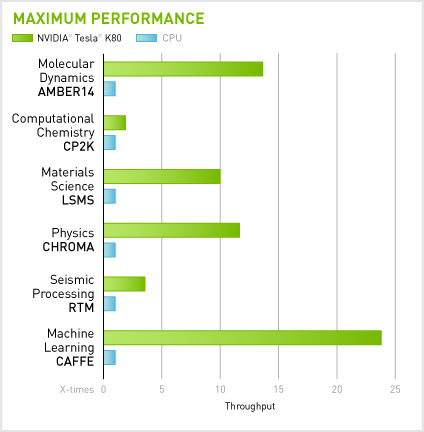
\includegraphics[width=.95\textwidth,height=0.7\textheight]{images/k80.jpg}
		    	\end{block}
		    \end{column}
		  \end{columns}
	\end{frame}

\section{Playing with code}

	\begin{frame}{Which frameworks to use?}
		\begin{columns}[T]
		    \begin{column}{.5\textwidth}
		    	\begin{block}{Tensorflow}
					\begin{itemize}
						\item Developed by Google
						\item Bindings in Python, Java, ...
						\item General purpose numerical framework
						\item Powerful, heavily tweakable
						\item GPU (CUDA) support
					\end{itemize}
		   		\end{block}
		    \end{column}
		    \begin{column}{.5\textwidth}
		    	\begin{block}{PyTorch}
		    		\begin{itemize}
						\item Python first approach
						\item Easy to get started
						\item Many examples and tutorials available
						\item GPU (CUDA) support
					\end{itemize}
		    	\end{block}
		    \end{column}
		  \end{columns}
	\end{frame}

	\begin{frame}{Basic structure of an ML script}
		The basic structure, which we're also using in our example code:
		\begin{itemize}
			\item Data preprocessing and loading
			\item Model definition
			\item Running and training
			\item Cross validation and logging
		\end{itemize}
	\end{frame}

\section{EOP}
\end{document}
